\documentclass[conference]{IEEEtran}
\IEEEoverridecommandlockouts
% The preceding line is only needed to identify funding in the first footnote. If that is unneeded, please comment it out.
\usepackage{cite}
\usepackage{amsmath,amssymb,amsfonts}
\usepackage{algorithmic}
\usepackage{graphicx}
\usepackage{textcomp}
\usepackage{xcolor}
\def\BibTeX{{\rm B\kern-.05em{\sc i\kern-.025em b}\kern-.08em
    T\kern-.1667em\lower.7ex\hbox{E}\kern-.125emX}}
\begin{document}

\title{Evaluating the Impact of Interactivity on User Engagement in Virtual Reality Museums: A Comparative Study}\\

\author{\IEEEauthorblockN{1\textsuperscript{st}I Putu Bagus Gede Prasetyo\\Raharja}
\IEEEauthorblockA{\textit{Department of Informatics} \\
\textit{Institut Teknologi Sepuluh Nopember }\\
Surabaya, Indonesia \\
6025231010@student.its.ac.id}
\and
\IEEEauthorblockN{2\textsuperscript{nd}Muhammad Shafhi Kasyfillah}
\IEEEauthorblockA{\textit{Department of Informatics} \\
\textit{Institut Teknologi Sepuluh Nopember }\\
Surabaya, Indonesia \\
6025231053@student.its.ac.id}
\and
\IEEEauthorblockN{3\textsuperscript{rd}I Nyoman Gde Artadana\\Mahaputra Wardhiana}
\IEEEauthorblockA{\textit{Department of Informatics} \\
\textit{Institut Teknologi Sepuluh Nopember }\\
Surabaya, Indonesia \\
6025231022@student.its.ac.id}
\and
\IEEEauthorblockN{5\textsuperscript{th}Hadziq Fabroyir}
\IEEEauthorblockA{\textit{Department of Informatics} \\
\textit{Institut Teknologi Sepuluh Nopember }\\
Surabaya, Indonesia \\
Hadziq@its.ac.id}
}

\maketitle

\begin{abstract}
The integration of virtual reality (VR) technology in museums presents opportunities to enhance user engagement and overall experience. This study evaluates the impact of interactivity on user engagement and system usability in VR museum settings, focusing on Balinese traditional masks. Two VR environments were compared: one with static displays and explanations, and another with enhanced interactivity and multimedia content. Results show that the interactive VR museum significantly improved user engagement and system usability, as indicated by higher System Usability Scale (SUS) scores and longer engagement times. These findings underscore the importance of interactive elements in VR educational tools for enhancing user experiences and learning outcomes.
\end{abstract}

\begin{IEEEkeywords}
Interactivity, Museum, User Engagement , Virtual Reality 
\end{IEEEkeywords}

\section{Introduction}
\IEEEPARstart{T}{he} integration of virtual reality (VR) technology in museums presents a significant opportunity to enhance user engagement, learning outcomes, and overall user experience. Previous research has shown that VR technology can enhance learning effectiveness and user experience by increasing perceived presence, immersion, realism, and satisfaction~\cite{10314973}​. However, these outcomes can vary significantly based on the level of interactivity and the design of the VR interface.

Museums worldwide have been adopting VR to create virtual tours, interactive exhibits, and digital archives. These VR applications aim to attract a broader audience, including those who cannot physically visit the museums. For example, Argentine museums have developed VR experiences that allow users to explore their collections from anywhere in the world~\cite{carvajal2020virtual}. Despite the growing popularity of VR in museums, there remains a need to understand how different levels of interactivity affect user engagement and learning outcomes.

This study aims to explore the effects of varying levels of interactivity in VR museum exhibits on user engagement, comprehension, and system usability, specifically focusing on exhibits featuring Balinese traditional masks. Balinese masks hold cultural and historical significance, often used in traditional dance performances and religious ceremonies~\cite{dadhich2016overview}. By incorporating these artifacts into VR exhibits, the study aims to not only preserve cultural heritage but also make it accessible to a global audience in an engaging manner. Two VR museum environments were developed for this study: one featuring static displays with plain sight explanations, similar to traditional museum exhibits, and another incorporating enhanced interactivity with features such as virtual manipulation of masks and multimedia content, including audio explanations. By comparing user experiences in these two environments, the study seeks to provide empirical evidence on the impact of interactivity in digital museums.

The research will employ quantitative methods to measure user engagement, comprehension, and system usability. Metrics such as time spent in the VR environments, questionnaire scores, and System Usability Scale (SUS) scores will be used to evaluate the effectiveness of each VR museum design. The findings are expected to contribute to the development of more effective and engaging VR educational tools, supporting the hypothesis that increased interactivity enhances user experiences and learning outcomes in VR museum exhibits.

This paper is structured as follows: Section II reviews related works on the integration of VR in museums and the role of interactivity in enhancing user engagement. Section III outlines the methodology used in this study, including the design of the VR environments, participant selection, and data collection procedures. Section IV presents the results and discusses the findings in the context of existing literature. Finally, Section V concludes the study and suggests directions for future research.

\section{Related Works}
The integration of virtual reality (VR) into educational and museum settings has generated substantial academic interest~\cite{7295086, 9590647, 9329425}. This section reviews key studies on the effectiveness of VR technology in enhancing user engagement, learning outcomes, and overall experience, with a particular focus on the role of interactivity. By examining these related works, the current study is contextualized within existing literature, highlighting the gaps it seeks to address.

Rahimi et al.~\cite{9286680} examine the impact of integrating virtual reality (VR) with physical exhibits in museums. Their research shows that VR-enhanced environments significantly boost learning and enjoyment compared to traditional and video-enhanced settings. By experimenting with different exhibit formats, the study provides valuable insights into how VR technology can create engaging and educational museum experiences, offering a promising direction for future hybrid museum spaces.

Kim et al.~\cite{6797425} discuss the development of an interactive VR interface for archaeological research and education. Focusing on the Northwest Palace of King Ashurnasirpal II in Iraq, the project integrates precise archaeological data into a VR environment, offering full-body immersion and user interaction with virtual artifacts. This VR museum aims to preserve and demonstrate cultural heritage, addressing the challenges of on-site conservation and providing a valuable tool for scholars and the public.

Guo et al.~\cite{9134304} present a comprehensive study on the evolution and application of digital interactive display technology in museums. Their research, showcased at the 2020 International Conference on E-Commerce and Internet Technology, delves into three main areas: three-dimensional laser scanning and modeling, multimedia information technology, and virtual reality interactive technology for displaying cultural relics. The paper highlights both the digital interactive display within existing museum spaces and the virtual interactive display for expanded spaces, providing insights into how these technologies enhance the visitor experience and preserve cultural heritage

Despite these advancements, there remains a need for more empirical research on the specific effects of varying levels of interactivity in VR museum settings. Most existing studies focus broadly on the benefits of VR without isolating the impact of interactivity. This study aims to fill this gap by providing a comparative analysis of static versus interactive VR museum exhibits. By focusing on Balinese traditional masks, this research will offer unique insights into how interactivity influences user engagement, comprehension, and overall user experience in a cultural heritage context.

\section{Methodology}

This study employs a comparative design to evaluate the impact of interactivity on user engagement and system usability within virtual reality (VR) museum settings. The primary focus is on examining two distinct VR environments featuring Balinese traditional masks. The first environment, termed the "Non-Interactive VR Museum," presents the masks in a static display format with plain sight explanations, akin to traditional museum exhibits. Users in this setting can navigate through the museum but cannot interact with the masks beyond viewing them and reading the provided descriptions. The second environment, referred to as the "Interactive VR Museum," enhances user interaction by allowing users to virtually hold and manipulate the masks. This setting also includes multimedia content such as audio explanations that provide historical context, usage in cultural ceremonies, and associated myths. By comparing these two environments, the study aims to investigate how varying levels of interactivity influence user engagement, comprehension, retention of information, and overall system usability.

\begin{figure}[htbp]
    \centering
    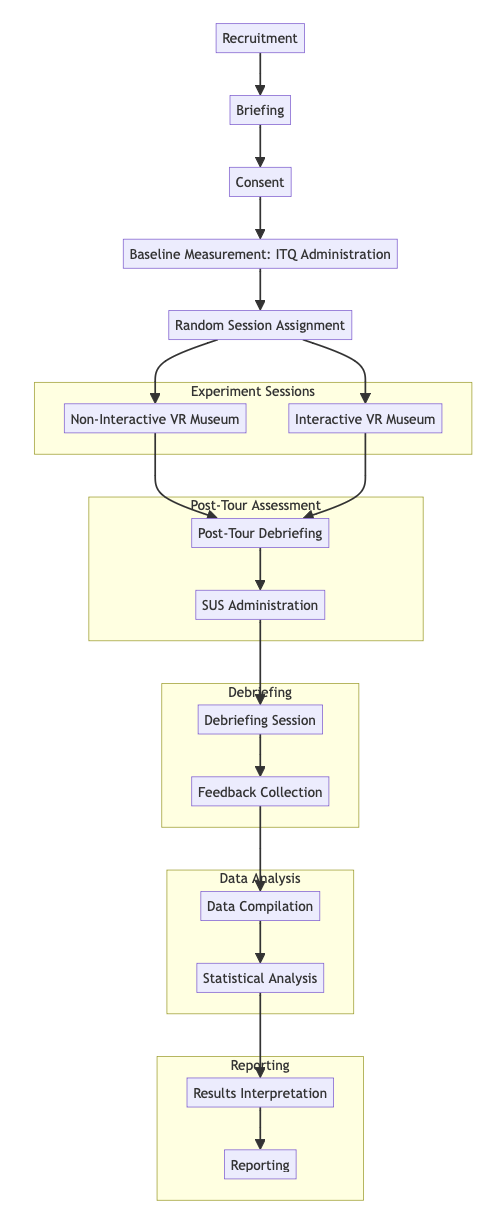
\includegraphics[scale=0.8]{Report/img/methodology.png}
    \caption{Research Flow}
    \label{fig:researchflowchart}
\end{figure}



\subsection{Participants}
Participants for this study will be Balinese university students majoring in Information Technology, aged between 20 and 22 years. This demographic is specifically chosen due to their likely familiarity with digital technologies and potential prior exposure to VR environments, making them suitable candidates for the study. The selection criteria include their age and educational background to ensure a consistent baseline of digital literacy and technical knowledge.

\subsection{Variables}
The independent variable in this study is the type of VR museum exhibit. This variable has two levels:

\begin{itemize}
    \item \textbf{Non-Interactive VR Museum}: This setting presents the masks in a static display format with plain sight explanations.
    \item \textbf{Interactive VR Museum}: This setting enhances user interactivity with the exhibits, including features such as the ability to virtually hold and manipulate the masks, zoom in for detailed textures, rotate the masks for different views, and access multimedia content including audio explanations.
\end{itemize}

The study focuses on two primary dependent variables to measure the outcomes of the different VR settings:

\begin{itemize}
    \item \textbf{User Engagement}: Measured by the time participants spend on each museum tour. Longer times are interpreted as indicative of higher engagement, particularly if the time is spent interacting with the exhibits in the interactive VR museum ~\cite{read2021engagement}.
    \item \textbf{System Usability}: Measured using the System Usability Scale (SUS)~\cite{vlachogianni2022perceived}, a 10-item questionnaire with responses ranging from "Strongly agree" to "Strongly disagree," resulting in a score from 0 to 100, with higher scores indicating better usability.
\end{itemize}

To ensure the consistency and validity of the results, several controlled variables will be maintained across both VR settings:

\begin{itemize}
    \item \textbf{Content Consistency}: The cultural and historical information provided about each mask will be identical in both settings to isolate the impact of interactivity.
    \item \textbf{Navigation Experience}: The navigation mechanics (e.g., movement through the museum space) will be consistent between the two settings to avoid confounding the results with differences in navigation ease or comfort.
    \item \textbf{Participant Demographics}: The study will target Balinese university students majoring in Information Technology, aged 20-22, to control for potential variations in background knowledge or familiarity with VR technology.
\end{itemize}

Confounding variables are factors other than the independent variable that might affect the dependent variable. Identifying and controlling for these variables is crucial to ensure the validity of the study's findings. In this study, potential confounding variables include:

\begin{itemize}
    \item \textbf{Immersive Tendencies (ITQ Scores)}: Immersive Tendencies (ITQ) scores indicate an individual's propensity to become deeply engaged in virtual environments~\cite{rozsa2022measuring}. Individual differences in immersive tendencies can influence how engaged participants are with the VR museum exhibits, regardless of the interactivity level. By measuring ITQ scores before the tours, these differences can be controlled for in the analysis to better isolate the effect of the VR museum type on engagement.
    \item \textbf{Order of Joining}: The sequence in which participants experience the interactive and non-interactive museums might influence their perceptions and engagement. For example, participants might be more engaged in the first experience due to novelty effects. Counterbalancing the order of joining and controlling for it in the analysis will help mitigate this potential confounding effect.
\end{itemize}
\subsection{Apparatus and Materials}
To conduct this study, the following apparatus and materials will be used:

\begin{itemize}
    \item \textbf{VR Headsets}: High-quality VR headsets such as the Oculus Rift or HTC Vive will be used to provide an immersive virtual reality experience for participants. These headsets will be used to display both the interactive and non-interactive VR museum settings.
    \item \textbf{VR Controllers}: Handheld VR controllers compatible with the VR headsets. These controllers will allow users to interact with the virtual objects, such as holding and rotating the masks in the interactive VR museum setting.
    \item \textbf{Questionnaires}: Digital versions of the Immersive Tendencies Questionnaire (ITQ) and System Usability Scale (SUS) questionnaires will be used to assess baseline immersive tendencies, usability, and other relevant metrics.
\textbf{    \item Environment Setup: A quiet room with minimal distractions will be set up where participants can use the VR equipment comfortably. This controlled environment is necessary to ensure that external factors do not influence the participants' experience or the study's results.} (buat penjelasan tentang environment (museumnya, dan asset topengnya lebih detail disini) (jangan pakai future tense, semua past tense karena sudah terlaksanakan)
\end{itemize}
\subsection{Procedures}
\subsubsection{Preparation}
\begin{itemize}
    \item \textbf{Recruitment}: Balinese university students majoring in Information Technology will be recruited for the study. Recruitment will be done through university channels, including announcements in classes, flyers, and emails.
    \item \textbf{Briefing}: Participants will receive a detailed overview of the study, including its purpose, what participation involves, the procedures to be followed, and any potential risks and benefits.
    \item \textbf{Consent}: Informed consent will be obtained from all participants. Participants will be informed about their rights, including the right to withdraw from the study at any time without penalty.
\end{itemize}
\subsubsection{Baseline Measurement}
\begin{itemize}
    \item \textbf{ITQ Administration}: Before the experiment sessions, participants will complete the Immersive Tendencies Questionnaire (ITQ) to assess their baseline immersive tendencies. This will help control for individual differences in how easily participants become immersed in virtual environments.
\end{itemize}
\subsubsection{Experiment Sessions}
\begin{itemize}
    \item \textbf{Session Assignment}: Participants will be randomly assigned to experience either the non-interactive or interactive VR museum first to counterbalance the order of exposure and control for potential novelty effects.
    \item \textbf{Non-Interactive VR Museum}: Participants assigned to this condition will explore the static VR museum with plain sight explanations. The time spent on the tour will be recorded to measure engagement.
    \item \textbf{Interactive VR Museum}: Participants assigned to this condition will interact with the VR museum using features like zooming, rotating masks, and accessing multimedia content. The time spent on the tour will be recorded to measure engagement.
\end{itemize}
\subsubsection{Post-Tour Assessment}
\begin{itemize}
\textbf{SUS Administration}: After each tour, participants will complete the System Usability Scale (SUS) to evaluate usability.
\end{itemize}
\subsubsection{Debriefing}
\begin{itemize}
    \item \textbf{Debriefing Session}: A debriefing session will be conducted to explain the study's purpose, answer any questions participants might have, and provide additional information about the research.
    \item \textbf{Feedback Collection}: Participants will be asked to provide feedback about their experiences in both VR museum settings. This feedback will be valuable for qualitative insights into the user experience.
\end{itemize}
\subsubsection{Data Analysis}
\begin{itemize}
    \item \textbf{Data Compilation}: Data from ITQ, time spent on tours, post-tour questionnaires, and SUS scores will be compiled for analysis.
    \item \textbf{Descriptive Statistics}: Calculate mean, standard deviation, median, and interquartile range (IQR) for each dependent variable in both groups.
\end{itemize}
\subsection{ANCOVA}

To evaluate the impact of the type of VR museum setting on user engagement, an Analysis of Covariance (ANCOVA) will be performed. ANCOVA, or Analysis of Covariance, is a statistical method that combines ANOVA and regression to compare group means while controlling for covariates. ~\cite{goldberg2020anova}. The formula for ANCOVA is as follows:

\[ Y_{ij} = \mu + \tau_i + \beta(X_{ij} - \overline{X}) + \epsilon_{ij} \]

where:
\begin{itemize}
    \item \( Y_{ij} \) is the dependent variable for the \( j \)-th observation in the \( i \)-th group.
    \item \( \mu \) is the overall mean.
    \item \( \tau_i \) is the effect of the \( i \)-th group.
    \item \( \beta \) is the regression coefficient.
    \item \( X_{ij} \) is the covariate for the \( j \)-th observation in the \( i \)-th group.
    \item \( \overline{X} \) is the overall mean of the covariate.
    \item \( \epsilon_{ij} \) is the error term for the \( j \)-th observation in the \( i \)-th group.
\end{itemize}

\subsection{Wilcoxon}
To compare the usability scores between the non-interactive and interactive VR museum settings, the Wilcoxon signed-rank test will be used. The Wilcoxon test is a non-parametric method for comparing two paired or independent groups.~\cite{kishore2022statistics}. The test statistic \( \ W \) is calculated as follows:

\[
W = \sum_{i=1}^n R_i^+
\]

where:
\begin{itemize}
    \item \( W \) is the test statistic.
    \item \( n \) is the number of paired samples.
    \item \( R_i^+ \) is the rank of the positive differences.
\end{itemize}

\subsection{Interpretation of Results} 
Interpret the results in the context of the study's hypotheses. The null hypothesis (H0) states that there is no significant difference in user engagement between the non-interactive and interactive VR museum settings after controlling for covariates. The alternative hypothesis (H1) states that there is a significant difference.

\begin{itemize}
    \item For ANCOVA, Evaluate the F-statistic and p-value to determine if there is a significant difference in user engagement after controlling for covariates.
\item For the Wilcoxon signed-rank test, Compare the test statistic to the critical value and p-value to determine if there is a significant difference in usability scores.
\end{itemize}
If the p-value is less than the significance level (typically 0.05), reject the null hypothesis in favor of the alternative hypothesis, indicating a significant difference between the groups.


\section{Results and Discussion}

The study aimed to compare user engagement and system usability in interactive and non-interactive museum settings, leveraging quantitative data collected via surveys and qualitative feedback. The dataset includes responses from participants regarding their depth of involvement in immersive experiences, which are critical in understanding engagement levels in different settings. Fifteen participants were involved in this study to assess the usability and engagement of both the interactive and non-interactive VR museum systems.

\subsection{System Usability Scale (SUS) Scores}
The SUS scores for both the interactive and non-interactive VR museum systems were collected to assess their usability. The descriptive statistics are as follows:
\begin{table}[h]
    \centering
    \begin{tabular}{|l|r|r|}
    \hline
                             & \textbf{Interactive System} & \textbf{Non-Interactive System} \\ \hline
    \textbf{Count}           & 15                          & 15                              \\ \hline
    \textbf{Mean}            & 41.93                       & 31.93                           \\ \hline
    \textbf{Standard Deviation} & 7.59                       & 7.53                            \\ \hline
    \textbf{Minimum}         & 30                          & 19                              \\ \hline
    \textbf{25th Percentile} & 35.5                        & 27.5                            \\ \hline
    \textbf{Median (50th Percentile)} & 40                 & 31                              \\ \hline
    \textbf{75th Percentile} & 50                          & 38.5                            \\ \hline
    \textbf{Maximum}         & 50                          & 42                              \\ \hline
    \end{tabular}
    \caption{SUS Scores for Interactive and Non-Interactive Systems}
\end{table}

A Wilcoxon signed-rank test was conducted to determine if there is a statistically significant difference between the SUS scores of the interactive and non-interactive systems:
\[
\text{Test Statistic} = 7.5, \quad \text{P-Value} = 0.00470
\]
Since the p-value is less than 0.05, we reject the null hypothesis, indicating a significant
difference between the usability scores of the interactive and non-interactive systems. This result suggests that the interactive VR museum system offers a significantly better user experience compared to the non-interactive system. The higher SUS scores for the interactive system indicate that users found it more user-friendly and engaging. This aligns with previous research suggesting that interactive systems tend to enhance user satisfaction and usability

User engagement was measured by the time participants spent in the VR museums. To control for potential confounding variables, such as participants' immersive tendencies (measured by the Immersive Tendencies Questionnaire, ITQ) and the order in which they experienced the VR museums, an ANCOVA was conducted. The results are summarized in Table~\ref{tab:ancova}.

\begin{table}[h]
\centering
\caption{ANCOVA Results for User Engagement}
\begin{tabular}{|c|c|c|}
\hline
\textbf{Variable} & \textbf{F-Statistic} & \textbf{P-Value} \\
\hline
Intercept & 50.28 & 0.022 \\
Museum Type & 14.68 & 0.001 \\
Order & 0.29 & 0.596 \\
ITQ Score & 0.01 & 0.905 \\
\hline
\end{tabular}
\label{tab:ancova}
\end{table}

\noindent The ANCOVA model summary is as follows:

\begin{itemize}
    \item R-squared: 0.362
    \item Adjusted R-squared: 0.289
    \item F-statistic: 4.924
    \item Prob (F-statistic): 0.00770
\end{itemize}

\subsubsection*{Coefficients}

\begin{itemize}
    \item Intercept: 50.28 (p = 0.022)
    \item Museum Type: 28.20 (p = 0.001)
    \item Order: -3.95 (p = 0.596)
    \item ITQ Score: -0.43 (p = 0.905)
\end{itemize}

The results indicate that the type of VR museum has a significant effect on the time spent by participants, with the interactive museum leading to longer engagement times. The p-value for the museum type is less than 0.05, suggesting a significant effect of the museum type on engagement time, even after controlling for ITQ scores and the order of joining.

These findings support the hypothesis that interactivity enhances user engagement. Participants spent more time exploring the interactive VR museum, indicating higher levels of engagement compared to the non-interactive VR museum. The ITQ scores and the order of joining did not significantly affect the engagement, showing that these potential confounders were effectively controlled.

\subsection{Implications}

The significant differences in SUS scores and engagement times between the interactive and non-interactive VR museum systems highlight the impact of interactivity on usability and user engagement. For developers and educators, this suggests that incorporating interactive elements can significantly improve the effectiveness of VR-based learning tools.

The findings of this study indicate that interactive VR environments can provide a more engaging and user-friendly experience. This has important implications for the design of educational VR applications, suggesting that features such as virtual object manipulation and multimedia content can enhance the learning experience and user satisfaction.

\section{Conclusion}

This study aimed to evaluate the impact of interactivity on user engagement and system usability within virtual reality (VR) museum settings, with a specific focus on Balinese traditional masks. By comparing two VR environments—one with static displays, plain sight explanations and the other with enhanced interactivity and multimedia content—the study sought to determine how different levels of interactivity influence user experiences. The findings provide valuable insights into the role of interactivity in enhancing the effectiveness of VR educational tools.

The results demonstrated that the interactive VR museum system significantly improved user engagement and system usability compared to the non-interactive VR museum. The interactive system received higher System Usability Scale (SUS) scores, indicating a better user experience. Additionally, participants spent more time in the interactive VR museum, reflecting higher engagement levels. These findings align with previous research suggesting that interactive systems enhance user satisfaction and usability. Key implications of this study include the importance of incorporating interactive elements in VR educational tools to improve user engagement and learning outcomes. Features such as virtual object manipulation and multimedia content were shown to be effective in enhancing the user experience.

these insights highlight the potential of interactive VR environments in creating more engaging and effective educational applications. Future research could extend these findings by exploring the impact of different types of interactivity and multimedia content in VR settings. Studies involving a broader demographic range and different cultural contexts could provide a more comprehensive understanding of the factors influencing user engagement and usability in VR educational tools.

\bibliographystyle{IEEEtran}
\bibliography{references}

\end{document}
